\documentclass{article}
\usepackage{math}
\usepackage{comment}

\title{Archimedes' Proof of Pi \\ 
\begin{large} 
Writing Assignment 2
\end{large}}

\author{Nicole Vivas}
\date{May 1 2025}

\begin{document}
\maketitle


% INTRODUCTION

\section*{Introduction}
% History: who was Archimedes\\
Archimedes de Syracuse (287 BC -212 BC) was one of the best mathematicians of his time. He transformed our understanding of geometry and gave us the first understanding of Pi and why it takes the form it does. From his work, he was able to find the first three digits of Pi, 3.14, the most crucial values, beginning the discovery of its infinite and patternless characteristics, which were found by future mathematicians.\\

%What led him to make this discovery\\
\textcolor{Periwinkle}{What led him to make this discovery?}
% FIRST SECTION 

\subsubsection*{Previous Understanding of Pi}

%Original knowledge of pi; Egyptian understanding and how he considered "The ratio of the circumference of any circle to its diameter as less than 3 1/7 but greater than 3 10/71."/ pi = C/D \\

In ancient Egypt, around 1650 BC, Babylonians had described Pi as the ratio od the circumference to the diameter, $\pi = \frac{C}{d}$. This is confirmed from the written document of 91 problems called the Rhind Mathematical Papyrus. They, inaccurately, (but pretty remarkably closely) calculated this value to be $\frac{256}{81}$ or roughly 3.1601. \\

\textcolor{Periwinkle}{add picture of the scribe}\\

\textcolor{Periwinkle}{also mention how this documented work was lost: 'It is claimed that in a text which is now lost, Archimedes gave better bounds whose average gives the value 3.141596 for $\pi$, correct to seven places.'}
%$ref: https://mathshistory.st-andrews.ac.uk/HistTopics/Pi_chronology/$

\section{Useful Definitions}
\textcolor{Periwinkle}{These defs are going to be mentioned in my own version of the proof}
\begin{definition}\label{def:TriArea}
The \textit{area of a right triangle} can be written as,\\
\[A_t = \frac{1}{2} b\cdot h\]
where $b$ is the base and $h$ is the height.
%area of a triangle
\end{definition}

\begin{definition}\label{def:apoth}
The \textit{apothem} of a regular polygon is the length of the line joining the center of the polygon to the midpoint of one of its sides. This is also the radius of the inscribed circle.\\

\begin{figure}[H]
    \centering
    \begin{minipage}{0.4\textwidth}
        \centering
        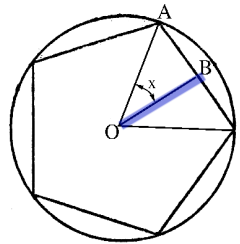
\includegraphics[width=0.5\linewidth]{circumscribed_apothem.png}
        \caption{Highlighted is the apothem of the circumscribed polygon.}
    \end{minipage}
    \hfill
    \begin{minipage}{0.45\textwidth}
        \centering
        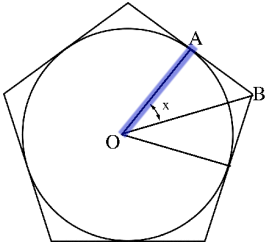
\includegraphics[width=0.5\linewidth]{inscribed_apothem.png}
        \caption{Highlighted is the apothem of the inscribed polygon. Note: This is the radius of the circle.}
    \end{minipage}
\end{figure}

\end{definition}

\begin{theorem}\label{thm:ipsum}

\end{theorem}


% SECOND SECTION

\section{Archimedes' Proof}
%Solving without modern geometry\\
Using prior knowledge of Pythagorean theorem, area of a triangle, and this fact of $\pi = \frac{C}{d}$ from the Egyptians, Archimedes proposed the idea of both inscribing a circle with a regular polygon of $n$ number of sides and circumscribing the same polygon; if we keep increasing $n$, we can get closer and closer to this value of what Pi should be. \\

%his proof/ how he went about the problem
In his writing, \textit{The Measurement of a Circle}, he wrote the revolutionary proposition:
\begin{proposition}
The ratio of the circumference of any circle to its diameter is less than 3 $\frac{1}{7}$ but greater than 3 $\frac{10}{71}$
\end{proposition}

For our proof, we will first look at the inscribed circle and find its perimeter \colorbox{Lavender}{(\ref{prt:1}) %I dont know why this is showing up as 2 and not 1%
} and then the circumscribed polygon's perimeter (\ref{prt:2}). \\

\begin{remark} \label{rmk:approx}
In this writing, without proof, Archimedes writes the approximate fractions of $\sqrt{3}$ stating it is between $\frac{1351}{780}$ and $\frac{265}{153}$. This was (assumed to be) found using an approximation formula of the form 
\[a\pm\frac{b}{2a} > \sqrt{a^2 \pm b} > a \pm \frac{b}{2a\pm 1}\] that he used, and was later defined by Heron of Alexandria and Al-Karaji as $\sqrt{a^2 + b} \approx a + \frac{b}{2a+ 1}$
\end{remark}

\begin{proof}
\,
\paragraph{I:} \label{prt:1}
Let $AB$ be the diameter of any circle, $O$ its center, and $AC$ the tangent at $A$. Let the angle $AOC$ be one-third of a right angle.\\

    Then, by the Pythagorean theorem, 
    \[OA : AC = \sqrt{3} :1\]
    By the approximation in \textit{Remark \ref{rmk:approx}}, 
    \[OA : AC > 265:153\]
    Thus,
    \[OC : CA = 2:1>306:153\]

    Let $OD$ bisect the angle $AOC$ and $D$ be on the tangent $AC$.\\

    Then,
    \begin{align*}
        CO:OA = CD:DA\\
        =CO+OA:OA = CA:DA\\
        =CO+OA:CA = OA:AD
    \end{align*}
    Then, using the approximation in \textit{Remark \ref{rmk:approx}},
    \[OA:AD>571:173\]
    To make it look like the Pythagorean theorem, we can write
    \begin{align*}
        OD^2:AD^2\\
        =(OA^2 +AD^2):AD^2\\
        >(571^2+153^2):153^2\\
        >349450:23409
    \end{align*}
    Thus,
    \[OD:DA>591\frac{1}{8}:153\]
    From this, Archimedes proceeded by bisecting the new angles, e.g. \textit{AO\textbf{D}}, which consequently duplicates the number of sides of the polygon. Thus,
    \[\begin{array}{c}
        OE:EA >1172\frac{1}{8}:153\\
        OF:FA > 2339\frac{1}{4}:153\\
    \end{array}\]
    
    If we have a fourth bisection $G$ then $AOG = \frac{1}{48}$(a right angle). \\
    
    Let there be an equivalent angle $AOH$ on the other side of $OA$ where $GA$ and $OH$ meet at $H$. Then $GOH = \frac{1}{48}$(a right angle). Thus, $GH$ is one side of a 96-sided regular polygon.\\

    Since $OA : AG > 4673\frac{1}{2}:153$, $AB=2OA$, and $GH=2AG$, observe the ratio:
    \begin{align*}
        AB : \text{\textit{perimeter of the 96-sided polygon}}\\
        >4673\frac{1}{2}:153 \times96\\
        >4673\frac{1}{2}:14688\\
    \end{align*}
    \begin{center}
        But,
    \end{center}
    \begin{align*}
        \hphantom{AB : \text{\textit{perimeter of the 96-sided polygon}}}\\
        \frac{14688}{4673\frac{1}{2}} = 3 + \frac{667\frac{1}{2}}{4673\frac{1}{2}}\\
        <3+ \frac{667\frac{1}{2}}{4673\frac{1}{2}}\\
        <3\frac{1}{7}  
    \end{align*}
    Therefore the circumference of the inscribed circle is less than $3\frac{1}{7}$ times the diameter AB.

\paragraph{II:} \label{prt:2}
let $AB$ be the diameter of a circle, and let $AC$, meeting the circle at C, make the angle $CAB$ equal to one-third of a right angle.\\

    Then, by Pythagorean theorem,
    \[AC:CB = \sqrt{3} :1 \boldsymbol{<} 1351:780\]

    Let $AD$ bisect the angle $BAC$ and meet $BC$ at $d$, and the circle at $D$\\

    From this, the angle $BAD = dAC$, thus, $=dBD$ and the angles at $D$ and $C$ are right angles, and the triangles $ADB, \,ACd, \,BCd$ are similar. \\

    Then,
    \begin{align*}
        AD:DB = BD : Dd\\
        =AC: Cd\\
        =AB: Bd\\
        =AB+AC:Bd+Cd\\
        =AB+AC:BC
    \end{align*}
    We also know,
    \begin{align*}
        AC:CB<1351:780 \: \text{while,}\\
        BA:BC = 2:1\\
        =1560:780
    \end{align*}
    \begin{center}
        Thus,
    \end{center}
    \begin{align*}
        AD:DB<2911:780\\
        \text{and} \: AB^2:BD^2 <(2911^2+780^2):780^2\\
        < 9082321: 608400\\
        \text{Thus,} \: AB:BD<3013\frac{3}{4}:780
    \end{align*}
    Repeating the process, we find the following:
    \[\begin{array}{c}
    AB:BF <1009\frac{1}{6} :66\\
    AB:BG<2017\frac{1}{4} :66
    \end{array}\]
    The fourth bisection of the angle $BAC$, the angle $BAG = \frac{1}{24}$(a right angle), therefore, $BG$ is one side of a 96-sided regular polygon. \\

    It follows that, 
    \begin{align*}
         \text{\textit{perimeter of the 96-sided polygon}}:AB\\
        > 96\times66:2017\frac{1}{4}\\
        >6336:2017\frac{1}{4}\\
    \end{align*}
    \begin{center}
        And,
    \end{center}
    \begin{align*}
        \hphantom{AB : \text{\textit{perimeter of the 96-sided polygon}}}\\
        \frac{6336}{2017\frac{1}{4}} 
        >3\frac{10}{71}  
    \end{align*}    

    By this calculation, the perimeter of a polygon larger than a circle must have a circumference of the circle greater than $3\frac{10}{71}$ times the diameter.\\

    Thus, the ratio of the circumference to the diameter is \textbf{less than} $3\frac{1}{7}$ but \textbf{greater than} $3\frac{10}{71}$. 
\end{proof}

\textcolor{Periwinkle}{Lemma: lets consider the same proof but with modern geometry}

\begin{theorem}\label{thm:ipsum}

\end{theorem}
% THIRD SECTION

\section{What this contributed to modern mathematics}

\textcolor{Periwinkle}{Foundational Constant for Geometry, Driving Force for Mathematical Development, blah blah blah}
% BIBLIOGRAPHY

\bibliographystyle{plain}  % see:  https://www.overleaf.com/learn/latex/Bibtex_bibliography_styles
\bibliography{vivasWA2}




\end{document}





































